\section{Vulnerability Classes and Notable CVEs}
\frame{\sectionpage}

\begin{frame}{Type Confusion}
    \begin{itemize}
        \item Type Confusion, CWE-843, is a class of vulnerability almost entirely unique to dynamically typed languages such as JavaScript.
        \item A highly exploitable vulnerability class, type confusions almost always lead to remote code execution within the browser sandbox.
        \item They occur as a result of accessing one JS object as if it were another. In V8, object access is determined by its \href{https://v8.dev/docs/hidden-classes}{\color{pink}HiddenClass}.
    \end{itemize}
    \begin{center}
        \begin{figure}
            \centering
            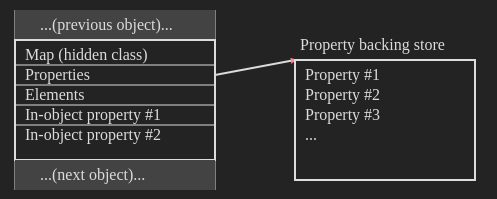
\includegraphics[width=0.5\textwidth]{images/v8-js-object.png}   
            \caption{The memory layout of a JS object, such as with `let v0 = \{\}`.}
            \label{fig:v8-js-object}
        \end{figure}
    \end{center}
    \note{
        \begin{itemize}
            \item Type Confusion is a child of CWE-704, "Improper Type Conversion or Cast"
            \item It is almost like halfway between a logical bug and a memory corruption bug. 
            \item Many bugs, despite not being type confusions, are said to be type confusions in Chrome's security bulletin. 
            \item There are many reasons why a type confusion may occur, but typically they occur due to incorrect graphs in Turbofan.
            \item A HiddenClass is also called a Map, but this has nothing to do with the JavaScript Map() class. 
        \end{itemize}
    }
\end{frame}

\begin{frame}{TheHole}
    \begin{itemize}
        \item TheHole is an internal memory sentinel used by the V8 Engine to represent out-of-bounds, uninitialized, or undefined values.
        \item Before Chrome 114, leaking TheHole into the JavaScript runtime was an extreme security risk. Nowadays, it would require a second vulnerability to fully exploit. 
        \begin{figure}
            \centering
            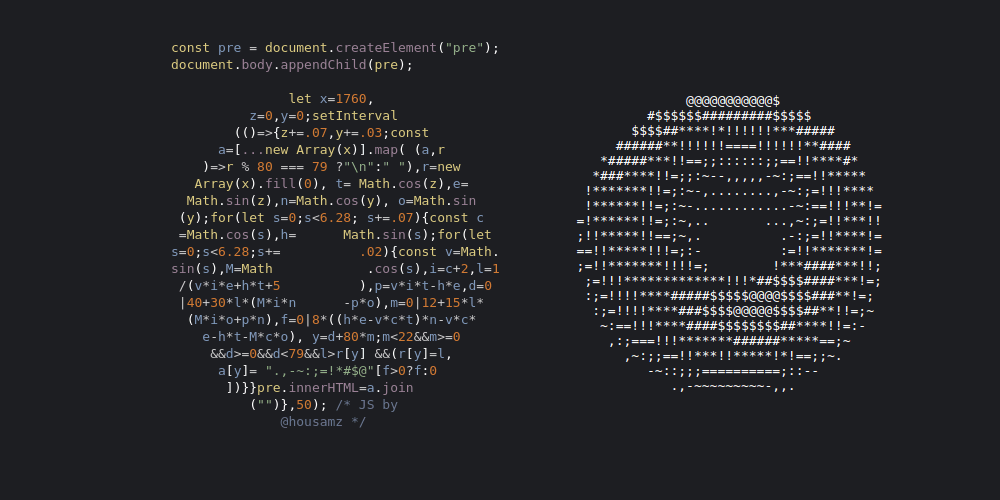
\includegraphics[width=0.55\textwidth]{images/v8-donut.png}
            \caption{A donut made with JavaScript, from Housam Ziad at hmz.ie.}
            \label{fig:donut}
        \end{figure}
    \end{itemize}
    \note{
        \begin{itemize}
            \item TheHole is exploitable for most of Chrome's existance, although the exploit pattern changes over time.
            \item The Chrome Developers didn't realize leaking TheHole was a security issue until Chrome 95 (2021).
            \item TheHole introduced an entire era of Chrome exploitation, lasting about two years (late 2021-2023).
        \end{itemize}
    }
\end{frame}


\begin{frame}{Insufficient Checks in Turbofan in "Array.at" -- BUG 1377775}{V8 Security Team -- Filed by Samuel "saelo" Gro$\beta$}
    \begin{columns}
        \begin{column}{0.5\textwidth}
            \begin{itemize}
                \item This bug runs the built-in function Array.at many times.
                \item Turbofan optimizes the code to expect these objects by inlining the function call to this built-in. 
                \item However, Turbofan only checks the kind of Elements, not the HiddenClass of the objects themselves. 
                \item This leads to a type confusion with "array" and "not\_array". 
            \end{itemize}
        \end{column}
        \begin{column}{0.5\textwidth}
            \usemintedstyle{vim}
            \inputminted{js}{code/buggy-bug.tex}
        \end{column}
    \end{columns}
    \href{https://bugs.chromium.org/p/chromium/issues/detail?id=1377775}{\color{pink}{crbug-1377775}}
    \note{
        \begin{itemize}
            \item This bug is an example of a type confusion. 
            \item The variable "not\_array", is identified by the engine as a JSObject. While "array" has the type JSArray.
            \item Both variables have the same kind of elements, "HOLEY\_ELEMENTS", meaning some members of their array-like backing are undefined. (For example array[1]).
            \item Array.at performs a lookup in the array at index "i". Turbofan sees this and determine that it doesn't need to make the function call to Array.at for the "bug" function. It can just do the lookup provided the types are correct.
            \item In reality, what TurboFan should do is bailout and deoptimize the "bug" function if it is called with exactly the wrong object type. 
            \item This bug was found quite quickly with automated testing and by fuzzing.
        \end{itemize}
    }
\end{frame}

\begin{frame}{Json.stringify Leaks TheHole Value, leading to RCE -- CVE-2021-38003}{Exploited in the wild by Variston -- Filed by Samuel "saelo" Gro$\beta$ and Clement Lecigne of Google TAG}
    \begin{columns}
        \begin{column}{0.5\textwidth}
            \begin{itemize}
                \item Likely the most canonical vulnerability in the history of Chrome, this bug was the first example of an exploit using TheHole. 
                \item The exploit was developed by Variston, a commercial spyware vendor in Barcelona. 
                \item JSON.stringify attempts to serialize a large value, but will ultimately generate an exception. V8 improperly handles the exception, causing an uninitialized value (AKA TheHole) to be returned.
            \end{itemize}
        \end{column}
        \begin{column}{0.5\textwidth}
            \usemintedstyle{vim}
            \inputminted{js}{code/json-stringify.tex}
        \end{column}
    \end{columns}
    \href{https://issues.chromium.org/issues/40057710}{\color{pink}crbug-40057710}
    \note{
        \begin{itemize}
            \item TheHole becomes leaked back into javascript objects most often by out-of-bounds reads. (e.g. bounds-check elimination).
            \item TheHole is a bit like a stack canary or a heap trailer, which are also memory sentinels. 
            \item Prior to Chrome 114, TheHole had an "OddballType" in the V8 engine. It shared this value with booleans and a few other built-in types.
            \item Notably, this allowed functions like toNumber() to be called on TheHole, which is very not good.
            \item Additionally, because of its use as a memory sentinel, other parts of engines were extremely not good at working with it.
            \item Nowadays, TheHole as a dedicated type. And trying to use it in any way causes V8 to halt and catch fire. 
        \end{itemize}
    }
\end{frame}

